\documentclass{article}
\usepackage[utf8]{inputenc}
\usepackage{setspace}
% \usepackage{verbatim}
\usepackage{fancyvrb}
\usepackage{graphicx}
\graphicspath{ {./images/} }
\usepackage{geometry}

 \geometry{
 a4paper,
 left=35mm,
 top=25mm,
 bottom=25mm,
 }


\doublespacing
\begin{document}
\newpage

% \maketitle
\section*{Chapter 1}
\section*{Introduction}


The term smart contracts, in an informal definition, can be interpreted as legal piece of agreement between two parties without the involvement of third party intermediators. Smart contracts represent a next step in the progression of blockchains from a financial transaction protocol to an all-purpose utility. They are pieces of software, not contracts in the legal sense, that extend blockchains utility from simply keeping a record of financial transaction entries to automatically implementing terms of multiparty agreements. Smart contracts are executed by a computer network that uses consensus protocols to agree upon the sequence of actions resulting from the contract’s code. The result is a method by which parties can agree upon terms and trust that they will be executed automatically, with reduced risk of error or manipulation. \\
Smart Contracts were first introduced by an American Scientist and Cryptographer, Nick Szabo, back in 1994. However, smart contracts gained popularity with the introduction of Ethereum, which uses the Solidity language to program the contracts. Bitcoin also supports smart contracts, but one must know opcode programming to use it. This makes smart contracts usage in Bitcoin very limited. But unlike Bitcoin, Ethereum can do much more. Developers can use Ethereum to build new kind of applications(dApps). The Ethereum community is the largest and most active blockchain community in the world. Thousands of developers all over the world are developing applications, and inventing new kinds of applications, many of which we can used today. Hence smart contracts on ethereum are increasing with a faster pace. Infact, the number of smart contracts deployed on the Ethereum network reached near 2M in March 2020. The total supply of Ether has crossed 100M mark in april 2020.\\
Smart contracts are immutable as long as blockchain integrity is not compromised. Since we cannot change smart contracts once deployed, any security vulnerabilities due to coding logic in the smart contracts will be visible to the public and cannot be patched. Hackers/attackers have exploited many such vulnerabilities in the past. Due to these exploitation's, damage of some million dollors worth ether happened already. The bigger issue is the trust of public. Suppose a company/developer deployed a faulty contract on ethereum and it is attacked, then the people no longer trust that company/developer. Hence during coding the developer have to be very careful and have to save his/her smart contract from exploitation atleast beacuse of the known vulnerabilities. To facilitate the developers, a good number of tools using various approaches, eg-static analysis, symbolic analysis etc are already built to check for various vulnerabilities. Every tools looks for specific set of vulnerabilites in the smart contracts. This thesis focused on the DoS vulnerabilities of the smart contract in our tool, DoS Tool. The main goal of this thesis is to build a symbolic analysis tool which will check for the Denial of Service vulnerabilities in the smart contracts.\\
The thesis is divided as follows: Chapter 2 provides background for various concepts necessary to understand the thesis work. Chapter 3 introduces various DoS vulnerabilites found in the past and existing related work related to denial of service. Chapter 4 introduces the symbolic execution approch for the Dos vulnerabilities and various DoS vulnerabilites patterns which are summarised from the DoS vulnerabilites explained in Chapter 3. Chapter 5 explains the working of the DoS Tool.
\newpage
\section*{Chapter 2}
\section*{Background}
\subsection*{Ethereum}
Ethereum was proposed in late 2013 by Vitalik Buterin, a cryptocurrency researcher and programmer. The development of ethereum was funded by an online crowdsale that took place between July and August 2014. The system then went live on 30 July 2015, with 72 million coins minted. Ethereum is an open source, blockchain based distributed computing system. Ethereum is the second largest cryptocurrency in terms of market capitalisation after the bitcoin.On Ethereum, we can write code that controls the money, and build applications accessible anywhere in the world. While all other blockchains also have the ability to process code, most are severely limited. Ethereum on the other hand rather than giving a set of limited operations, it allows developers to create whatever operations they want. This opens a wide area to explore and we can see more exciting and innovative Apps and concepts on ethereum. For example we can develop games, manage financial transactions, building multi party system and many more. 
\\ 
Smart contract on ethereum can let developers and organisations to code their Apps( called as Distributed Apps because they are built on distributed network, ethereum). These smart contracts are like computer programs and execute the exact functionality/logic using EVM. These apps once deployed is opened to public and cannot be tampered with because of the blockchain property and because of this ethereum is growing rapidly in popularity. Increasing numbers of organizations are embracing Ethereum for new projects. The variety of projects that use Ethereum as their foundation is almost limitless. 
The State of the dApps website shows how many Ethereum projects exist in different categories and how popular they are. Some sample examples of how ethereum can be used:\\
\begin{itemize}
    \item Gnosis and Augur are many of the innovative companies using ethereum in interesting ways. Both provides a platform for the prediction markets. Users use company specific tokens to predict and and wins token for successful predictions. These predictions are useful for the others who are looking for investment in stocks etc.
    \item We can also find some games in the ethereum space as. Cryptokitties is one of the ethereum first games which is still popular. The game introduced blockchain-based cryptocollectibles. Cryptokitties are breed from the cattributes of their parents. The popularity of games can be seen from the fact that some of the cryptokitties are sold for over \$10000 USD in the past.
    \item  Ethereum platform is also used to make social platform to share thoughts. EtherTweet is the blockchain based alternative to twiter.
    \item Ethereum can be used to search for jobs using EthLance. EthLance is a distributed platform for freelancers and employers to find each other, engage in jobs, and transfer payment in ether and so on.
\end{itemize}
and many more...\\

The transaction rate on ethereum is around 7-8 lakhs per day. The total supply of Ether was around 100 million as of 16 April 2020 and around 2M smart contracts already deployed on ethereum. With so many smart contracts deployed and money involved, attracts the attackers to find and exploit vulnerabilities in the smart contracts. We have seen many vulnerabilities in the past because of which there was huge loss of money/ether. Few famous vulnerabilites are listed below.
\begin{itemize}
    \item The reentrency attack is among the most famous on ethereum. Reentrency occurs when a external called contract is allowed to make call to the calling contract without completing the previous execution. The famous DAO attack is an example of the reentrency attack which cost around 50USD at the time.
    \item Access control issues which allowed any external user to perform privilege operations. One usually access these access through the public or external functions and insecure visibility settings gives direct opportunity to attackers. This vulnerability costed around 30M USD at the time. The real world impact due to access control are Parity Multi-sig Bug 1, Parity Multi-sig Bug 2 and Rubixi etc.
    \item Denial of service is dangerous in the world of Ethereum. While other types of applications can eventually recover, smart contracts can be taken offline forever by just one of these attacks. There are many ways that lead to denials of service, these include maliciously behaving when being the recipient of a transaction, increasing the gas necessary to compute a function , abusing access controls to access private components of smart contracts, taking advantage of mixups and negligence, etc. This class of attack includes many different variants and will probably see a lot of development in the years to come. The total estimated loss because of Denial of Service is around 300M USD at the time. Real world impact/ examples are GovernMental[], King of Ether contract and Parity Multi-sig Wallet etc.
\end{itemize}  

\subsection*{Smart Contracts}
Smart contracts are terms and conditions which the two parties agreed upon before doing business with each other. These enforce these terms and conditions programatically and thus removes middle man who in the absence of smart contract is the main enforcer of the terms and conditions. The middle man sometimes can favour one person over the other and can change the terms and conditions in order to get some money or cheat the other person. Smart contract reduces this fraud and removes the issue of trust because this are computer programs which runs exactly programmed and cannot be changed if they are implemented on blockchain. Example : Ethereum Smart Contracts etc. A smart contract can work on its own and it can also be implemented along with any number of smart contracts. For example a smart contract can be called from other smart contract, successful completion of one contract can triger the second and so. We can make the complete organisation run on smart contract. \\
Smart contracts gives a number of benefits. Smart contract eradicate the need of third party involved in the transaction. They provides trust as no one can steal them and are stored on public ledger which can be seen by everyone and are verified by 100's or 1000's of nodes. Smart contracts save money by eliminating the notary, estate agents, assitances etc charges. Smart contracts, if implemented correctly, provides safety as these are very hard to hack. Smart contract also save a lots of time which will otherwise be wasted on manually processing lots of paper work,  sending and receiving transportation time etc.\\
Smart contracts were first proposed in the early 1990s by computer scientist, lawyer and cryptographer Nick Szabo. However the implementation of smart contracts did not happen until 2009, when the first cryptocurrency blockchain bitcoin came and provides suitable environment for the implementation of smart contracts. But their implemntation still is very much regulated and controlled by the bitcoin. But with the arrival of ethereum, the smart contract gets more freedom because of the turing completesness of EVM and become the most hyped feature of ethereum. Smart contracts can now implement almost all the practical life examples.\\
Smart contracts are extremely new technology. Despite of so many attactive promises, they can still be prone to problems. The code of the smart smart contract logic must be accurate and contains no bugs. This can lead to mistakes and most of the time are exploited by attackers for the wrong doing to the system/ smart contracts. For example the DAO hack, King of Ether vulnerability are the examples of ethereum smart contracts where scammers found vulnerabilities in the smart contract logic and exploited them.
\subsection*{Ethereum Smart contract Programming}
Any program that runs on the Ethereum Virtual Machine (EVM) is commonly referred to as a smart contract. The most popular languages for writing smart contracts on Ethereum are Solidity and Vyper. Solidity is the most popular language on ethereum, inspired by C++, python and javascript. Vyper is based on python. The IDE's for the ethereum developments are Visual Studio Code with official ethereum support, Remix is a web based IDE with built in static analysis, and a test blockchain virtual machine and EthFiddle is also an web based smart contract to write, compile and debug smart contracts. We have used Remix to generate bytcode for our sample test smart contracts.
\subsection*{ByteCode}
When we compile the high level smart contract code, say for example a solidity file on Remix, it will translate the high level code into the bytecode. The bytecode is a hexadecimal representation of the smart contract. Since this bytecode will run on the EVM, the EVM have predefined opcodes. The bytecode contains these opcodes into their hexadecimal values. Every opcode have a hexadecimal values. The mapping of hexadecimal values to the opcodes can be seen in the ethereum yellow paper and here. EVM is a stack based machine and every opcode take arguments from the stack and processes on those arguments and put back the result on the stack. There are some opcodes which puts data on the stack without processing. Lets look at these opcodes below.
\begin{itemize}
    \item \textbf{Opcodes of execution environment}: For example PC for program counter and MSIZE for current memory size.
    \item \textbf{Opcodes for transaction}: These are the opcodes that contain details about the transaction payload used to call smart contract, for example, CALLVALUE stores the ether value sent along with the transaction, CALLDATASIZE returns the size of CALLDATA(transaction payload) etc.
    \item \textbf{Opcodes to push constant values on the Stack} : These opcodes push constant values on the stack to process further.For example, PUSH opcode that pushes value on the stack. The PUSH opcode can push different bytes of data on the stack base on the prefix number attached to the PUSH. For example PUSH1 pushes 1 byte of data onto the stack, PUSH8 pushes 8 byte of data onto the stack and so on. The highest value that can be pushed on the stack is of 32 bytes by PUSH32. there is no PUSH33 and above. 
\end{itemize}
The recent 16 values on the top of the stack are accessible because of which we have opcodes for duplicate and swap stack values with prefix DUP1...DUP16 and SWAP1...SWAP16.\\
There are certain opcodes used for identifying symbolic variables in the bytecode. These opcodes are basically those which are to to process data about the CALLDATA. CALLDATA is the transaction payload string that is send as transaction to call a contract. This string is send as transaction to call a contract. External users interact with the smart contracts on ethereum blockchain this way. A list of opcodes for processing the CALLDATA is listed below.
\begin{itemize}
    \item \textbf{CALLVALUE} : CALLVALUE stores the ether value send by the calling contract. This is decided by the external user who is calling the contract and hence we treated this value as symbolic.
    \item \textbf{Calling External Contract from the Contract} : The return value of calls made to external contract from the contract are purely symbolic as we don't know the external smart contract. It is generally a boolean value for successfully completion of the execution of external smart contract or for the failure of executtion of the external smart contract. The opcodes for calling external smart contracts are CALL, CALLCODE, DELEGATECALL and STATICCALL.
    \item \textbf{CALLDATALOAD(x)} : The opcode CALLDATALOAD(x) is used for loading a specific part of the CALLDATA string strating from xth byte upto 32 bytes either for the purpose of loading external function signature in the payload string which the user want to call in the smart contract or for the function arguments provides in the payload string to call the particular functions. As these are purely set by the caller the smart contract don't know what value is coming in the payload and hence we set all these as symbolic.
    \item \textbf{CALLDATACOPY(t, f, s)} : CALLDATACOPY(t, f, s) copies \emph{s} bytes from calldata at position \emph{f} to memory at position \emph{t}. These bytes stored in memory are all stored as symbolic variables.
    \item \textbf{CALLDATASIZE} : CALLDATASIZE returns the size of the calldata in bytes is also treated as symbolic.
\end{itemize}
    
There are two types of bytecode:
\begin{itemize}
    \item \textbf{Creation Bytecode} : When a smart contract is compiled creation bytecode is generated. This is the code that generates runtime bytecode. It contains contructor logic and constructor parameters of a smart contract. This code sets the initial parameters using constructor and returns the runtime bytecode which is actual smart contract. The creation bytecode is equivalent to the payload of the transaction the creates a contract, provided the sole purpose of the transaction is to create the contract.\\

    The creation bytecode for a contract can be retrieved on-chain by using
    \begin{center}
        \emph{type(ContractName).creationCode}
    \end{center} 
    \item \textbf{Runtime Bytecode} : Runtime  Bytecode is the code that is stored on-chain that describes a smart contract. This code does not contain constructor logic and constructor parameters as these are not relevant to the smart contract once it is deployed on the blockchain. \\
    The runtime bytecode for a contract can be retrieved on-chain by using an assembly block and calling
    \begin{center}
        \emph{extcodecopy(a)}
    \end{center} 
    And the hash of the runtime bytecode is returned from 
    \begin{center}
        \emph{extcodehash(a)}
    \end{center} 
\end{itemize}
\subsection*{Ethereum Virtual Machine(EVM)}
Virtual machines are essentially creating a level of abstraction between the executing code and the executing machine. This layer is needed to improve the portability of software, as well as to make sure applications are separated from each other, and separated from their host. All nodes in the ethereum network agree on how should EVM behave. This helps in achieving concensus for the data and the code on the code as everyone will get the sam data due to their agreement on EVM.\\
EVM is a stack based machine with the maximum limit of the stack is 1024. EVM also keeps track of the gas usage in order to terminate program when out of gas. In this thesis we implemented a Cutom EVM which only executes bytecode instead of implementing fully functional EVM. Hence a knowledge of all storage components is sufficient. he Ethereum virtual machine specification lists three separate storage as listed below:
\begin{itemize}
    \item \textbf{Stack} : EVM is a stack based machine. The stack is the area where all general purpose computation happens. The stack size can goes upto a maximum of 1024. If a contract reaches this stack size the EVM stops execution of the contract. The stack can hold upto a maximum of 32byte of data item. Stack is the cheapest memory in terms of gas consumption.
    \item \textbf{Memory} : Memory is linear and holds temporary variable because memory is temporary and erased between function calls. Memory can be seen as an additional assist to the stack computation for the execution of the current call. The maximum bytes of data that can be read at one time from a memory is 32 bytes. We can write from a range of 8bit to 256bits of data on the memory. To expand memory from a default size one needs to pay extra gas. Memory scales quadratically and the more it grows, more it costs. 
    \item \textbf{Storage} : Storage is used to store smart contract's state. This is permanent between function calls. The gas consumption is highest of all the three memory in case of storage.
\end{itemize}
\subsection*{Control Flow Graph}
Control flow graph is a representation, using graph notations, of all the paths that a program might traverse during its execution. Each node in the control flow graph is called as a basic block. Directed edges are used in the control flow graph to show the control flow from one basic block to another. The control flow graphs can be used to detect loops, detect various control structures, for example, loops, if-the-else etc in the program. 
\subsection*{Denial of Service}


\newpage
\section*{Chapter 3}

\section*{DoS Vulnerabilities in Ethereum Smart Contracts}
There are few DoS attacks/vulnerabilities found in the past which exploit smart contract vulnerabilities.\\
\\
\textbf{King of Ether Smart Contract}\\
In 2016 this contract was deployed. It was a game where players send ether to the contract to take the throne. The new player claims the throne whenever he/she send more ether. If 14 days passed and there is no new successors, the throne was reset and game started all over again. The idea is every successor have to pay more ether than the previous successor in order to take the throne. Hence value of throne increases with more and more successors. The contract's function to update the successor looks similar to the code below.

\begin{Verbatim}[numbers=left,xleftmargin=5mm]
contract setThrone {
    
    address currentSuccessor;
    uint highestValue;

    function claimThrone() payable {
        require(msg.value > highestValue);
        require(currentSuccessor.send(highestValue)); // Refund the old Successor else revert

        currentSuccessor = msg.sender;
        highestValue = msg.value;
    }
}
\end{Verbatim}
The problem in the contract is with the statement\\
\\
\emph{require(currentSuccessor.send(highestValue));}\\
\\
The \emph{address.send()} have a gas limit of 2300 gas. While this is good to prevent reentrency bug but this limit of gas will result in failure to send the ether to the previous successor's contract if the player's(previous successor's) fallback function consumes more than 2300 gas. Hence the player can claim throne and then fails the send command purposely so that no new player can claim throne even if the new player is eligible to claim the throne. This results is denial of service of the contract by rejecting new thrones even if eligible.\\
\\
\textbf{Block Gas Limit}\\
Each block has a limit on the amount of gas spent. If the amount of gas spend exceeds the limit the transaction will fail. Hence this transaction can never be added into the blockchain. This will lead to the denial of service since that contract will no longer work as this transactions will not be added into the blockchain. Unbounded loops are the cause for this vulnerability. If the attacker can manipulate the loop limit, he/she can manipulte the amount of gas spend within the block. There are two primary ways to make loops unbounded.\\
\begin{enumerate}
    \item Let's consider the below smart contract
    \begin{Verbatim}[numbers=left,xleftmargin=5mm]
    pragma solidity ^0.4.24;
    
    contract BasicToken {
        uint256[] balances;
        
        function add(uint256 a) private  {
            balances.push(a);
        }
        function balanceOf() public  view returns (uint256) {
        
            uint c = 1;
            add(i);
            return c;
        }
        function print() public view returns (uint256){
            uint256 temp = 0;
            for(uint256 i = 0; i < balances.length; i++){
                temp += balances[i];
            }
            return temp;
        }
    }
    \end{Verbatim}
    
    The \emph{balanceOf()} function in the above contract let anyone add items to the \emph{balances} array. Then in the \emph{print()} function the loop condition is on the length of the \emph{balances}. An attacker can intentionally add garbage values to the \emph{balances} array and then \emph{print()} function will exceeds the block gas limit. Hence the transaction containing \emph{print()} function call will always fail when the \emph{balances} array length reach a certain limit. Hence \emph{print()} function will become unavailable. 
    \item Changing loop length directly\\
    The iteration of loops can be on a constant value, or an variable, or dynamic array, or mapping. All of these other than the constant value can be changed directly by assigning value to it by assigning a direct value. If such assignment statement is controlled by external user then it could lead to vulnerable loop.\\
    \\
    For example the following statement in the above smart contract\\
    \emph{balances.length = \textbf{arbitrary value}}\\
    \emph{\textbf{arbitrary value}} is given as argument to \emph{balanceOf()} function.\\
    
    
\end{enumerate}
It is to be noted that these conditions for making loops unbounded could be made accessible only to some allowed addresses. These addresses are decided by the owner of the smart contract for example if the above smart contract is change as below. Line 6-13 are added in the above smart contract. An variable \emph{owner} of type address is added. The value of \emph{owner} is set in the constructor. \emph{modifier onlyowner()} checks whether the caller address is same as owner. If both the addresses matches then the program proceeds further else revert. Now even if the \emph{balanceOf()} function is called by anyone, the call from the owner address will proceeds further. All other addresses(other than owner) which try to take benefit of \emph{balanceOf()} function will fail. Even though this will also result in denial of service for the \emph{print()} function, this case should not be considered as a vulnerability because no outsider is able to exploit the denial of service vulnerability. Maybe the coder is aware of such behaviour and still he wants to code this contract. Hence we cannot be sure of the intent of the coder and therefore this thesis will focus only on the cases which can be exploited by the the attackers. 

\newpage
\begin{Verbatim}[numbers=left,xleftmargin=5mm]
    pragma solidity ^0.4.24;

    contract BasicToken {
       uint256[] balances;
       
       address owner; // owner address
       constructor(address o) public { // constructor to set owner
           owner = o;
       }
       modifier onlyowner(){ // modifier to check if caller is owner else revert
           if(msg.sender != owner) throw;
           _;
       }
    
       function add(uint256 a) private  {
           balances.push(a);
       }
       function balanceOf() public  onlyowner view returns (uint256) {
           uint c = 1;
           add(i);
           return c;
       }
       function print() public view returns (uint256){
           uint256 temp = 0;
           for(uint256 i = 0; i < balances.length; i++){
               temp += balances[i];
           }
           return temp;
       }
    }
\end{Verbatim}
\newpage
\section*{CREATE2 Information Leak Vulnerability}
An exploitable information leak / denial of service vulnerability exists in the libevm ( Ethereum Virtual Machine ) \emph{CREATE2} opcode handler of CPP-Ethereum. The attacker can create smart contract to triger this vulnerability. Hence use of \emph{CREATE2} vulnerability should be considered as denial of service vulnerability.

\section*{Existing related work on DoS}
\begin{itemize}
    \item \textbf{An Adaptive Gas Cost Mechanism for Ethereum to Defend Against Under-Priced DoS Attacks} proposes a novel gas cost mechanism, which dynamically adjusts the costs of EVM operations according to the number of executions, to thwart DoS attacks. 
    \item \textbf{SmartCheck: Static Analysis of Ethereum Smart Contracts} is a static analysis tool which looks for conditional statements (if, for, while ) containing condition as an external call. This tool also looks for the unbounded loop.
    \item \textbf{Slither – a Solidity static analysis framework} is another static analyzer where external calls in loops is considered as one of the vulnerability. 

\end{itemize}

\newpage
\section*{Chapter 4}
\section*{A Symbolic Approach to find DoS Vulnerabilities in Ethereum Smart Contracts}


Symbolic execution is a means of analyzing a program based on the inputs that the program can take and paths that can be traversed because of different inputs. Suppose we have a function with arguments which can be called by external user. These arguments will be of some types for example integer, string, boolean, etc. Every type have some range of sets of value that can be assigned to variable. Hence the external user have a set of choices which he can use while calling the function. Hence instead of testing the program on some random fixed inputs every argument is considered as symbolic variable. The program execution will go on as normal and when the argument is used in some computation during the execution of the program the symbolic variable will used. This will generate symbolic expression as the program execution proceeds. This symbolic expression/variable can be used to resolve the condition branch to decide logically whether certain path from the current execution point is reachable or not. A symbolic execution is shown in the example below
\begin{Verbatim}[numbers=left,xleftmargin=5mm]
    pragma solidity ^0.4.24;
    contract BasicToken {
    function fun(uint256 s) public  view returns (uint256) {
        uint c = s; /*/ c = sym
        c = s + 1; /*/ c = sym + 1
        for(uint i = 0; i < c; i++){ /*/ for(uint i = 0; i < sym + 1; i++){
            // some code
        }
        if(c > 10){ /*/ if(sym + 1 > 10){
            //some code
        }
        else{
            //some code
        }
        return c;
    }
}
\end{Verbatim}
In the above example the variable \emph{s} is symbolic because \em{fun} is an external function in solidity and can be called by whoever wants to interact with the smart contract using the \emph{fun} function. The function also has an argument that is to be supplied by the caller through transaction payload that is used to call the function. The symbolic execution of the function will treat \em{a} as a symbolic argument. On assignment of symbolic variable on line 4, the local variable will be assigned a symbolic value, \em{sym}. Line 5 of the codes do some processing with the symbolic variable and hence a symbolic expression is the result of the processing, \em{sym + 1}. Now this symbolic expression if used for branch decision, then it will be feed to the SMT solver in order to symbolically decide which branch which path to traverse. There may be possibility to traverse all the paths or one path according to the satisfiability of the symbolic expression. For example, loop condition on line 6 is satisfiable for both the paths, loops can be traversed for the condition $i >= sym$ and loop can break for the condition $i < sym$. Similarly on Line 9 of the code if condition is satisfied for $sym >= 10$ and not satisfied for $sym < 10$.\\
Hence in order to find DoS vulnerabilities we will execute all paths of a smart contract which can be traversed symbolically and check for vulnerabilities patterns as discussed below during the execution of the smart contract.\\
\\
\subsection*{Vulnerability Patterns}
\begin{itemize}
    \item \textbf{Call to address changed by attacker}\\
    An attacker is able to change the address of the external call made from the victim contract. This ability may be the functionality of the contract as we have seen in the chapter 3. But this can be used against the victim contract. The attacker can purposely and deliberately code his fallback function in such a way that the call will never be executed successfully. Now there will be multiple scenarios
    \begin{itemize}
        \item \textbf{Exception check on the call in victim contract}\\
        The failed call will revert the execution of the victim contract and hence the particular function will throw an exception and the execution of the victim contract will stop every time the particular function containing such call is invoked. This will make every execution trace containing such calls revert and become unavailable for use.
        \item \textbf{No exception check on the call in the victim contract}\\
        The inbuilt functions \emph{send() and call()} do not throw exceptions by themselves, instead they must be handled manually. In case they are not handled then the \textbf{King of Ehter} contract will execute normally and only the attacker will be in loss because he is removed from the throne and the ether he invested also lost due to the failed call. But these functions return values for example call return 1 on success and 0 on fail. There could be some computations based on this return value. Now even though there is no exception and nobody knows if there is anything wrong, the path of execution which is supposed to be executed on the success of the call will never be reached. Hence this can also lead to denial of service if the logic of the smart contract permits.
        \item \textbf{variable gas limit in \emph{call()} function}\\
        The \emph{send() and transfer()} function have gas limits and are easy to exploit for the DoS attack in the above scenario. But the \emph{call()} function have the option to set the limit of gas to be send to the called contract. But this will not pose any serious threat to the vulnerability as the attacker can try different gas limit fallback function to consume all the gas.
    \end{itemize}
    Hence if on traversing any execution trace we came across a \emph{call()} function whose \emph{address} argument is symbolic variable or symbolic expression, the tool flag the contract as vulnerable.\\
    \item \textbf{Loop with Symbolic Variable Condition}\\
    Ethereum have a block gas limit. If a block consumes more gas than the limit then the execution stops and the transaction reverts. Hence this path of execution will never be completed and hence the denial of service. If the conditional expression is symbolic variable/expression it can take different values and can lead to block gas limit. Please note that loops with conditional expressions as fixed can also reach the block gas limit if the the fixed value is large enough. But this block gas limit will be from start of the deployment of code on ethereum and no malicious person is needed to invoke that vulnerability.Hence the loops with conditional expressions as symbolic variable/expressions are considered as vulnerable.
    
    \item \textbf{Call to address changed by attacker in loop}\\
    This is no different vulnerability. It is the same as \emph{Call to Address Changed by Attacker} but inside the loop. There is no condition on loop. It can be with the conditional expression as fixed value or it can be with the conditional expression as symbolic variable/expression.
    \newpage
    \item \textbf{CREATE2 Opcode}\\
    An exploitable information leak / denial of service vulnerability exists in the libevm ( Ethereum Virtual Machine ) \emph{CREATE2} opcode handler of CPP-Ethereum. Hence if in the bytecode \emph{CREATE2} opcode id found we considered it as vulnerable.
\end{itemize}

\newpage
\section*{Chapter 5}
\section*{Working of Tool}
An ethereum smart contract after compilation generates bytecode. This byecode is deployed on the ethereum blockchain. The source code is not stored on blockchain. Hence there is no way to know the source code of a deployed smart contract. Etherscan is a Block Explorer, Search, API and Analytics Platform for Ethereum. Among other things they also provide the source code verification as a service. Anyone can use this service to attach a source code with any deployed smart contract. The tool build the deployment payload and check if the same payload is on blockchain or not. If both matches then the source code is linked to the payload on etherscan. Hence we can find source code of many smart contracts on etherscan. Since there are millions of smart contracts deployed on blockchain not all smart contract's source code can be found on etherscan. But for the working of our tool we only need bytecode of smart contract instead of source code. The bytecode of a smart contract is given as input to the DoS Tool, it processes the bytecode and generates the output as shown in the figure below.\\
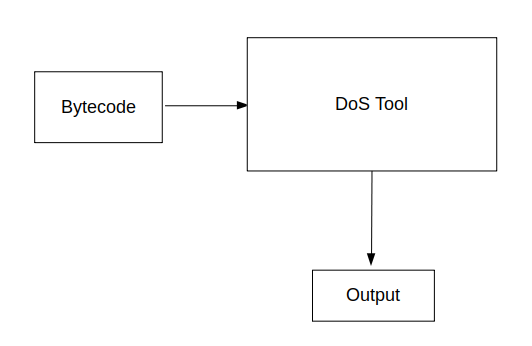
\includegraphics[width = 15cm, height = 10cm]{images/1.png}
\begin{center}
    Figure 1
\end{center}
The output of the DoS tool will print the respective vulnerabilities as discussed under the topic Vulnerabilities Patterns in chapter 4.

\newpage
\noindent \textbf{Insight of Components of DoS Tool}\\
We will now dive deep into DoS Tool working. The bytecode is feed to the \textbf{\emph{parser}} which preprocess the bytecode. The \textbf{\emph{parser}} converts bytecode into opcode view named as parsed code in the tool. These opcodes and the control flow graph are feed to the \textbf{\emph{Symbolic Execution Phase}} which is the Custom EVM executed symbolically. The Symbolic Execution Phase along with the ouput also update a list of visited nodes. These list of visited nodes are the nodes that can be visited during the execution of Symbolic Execution. Hence these list of nodes are a subset of the nodes present in the Static CFG. The \textbf{\emph{Symbolic Execution Phase}} also resolves new paths which were not able to be resolved statically. This path resolution will be discussed in detail. Using the visited node list we update the Static CFG by deleting the nodes from the CFG which are not present in the visited node list. The gaph algorithms to find elementary cycles are used to find loops in the updated CFG.The \emph{Updated CFG} is used to find the number of paths that can be traversed. The numbers in most cases should not match with the number of paths found in Static CFG because of overestimation of paths. This will be discussed in the subsequent topics. A flow diagram of the DoS Tool is shown in the Figure 2.\\
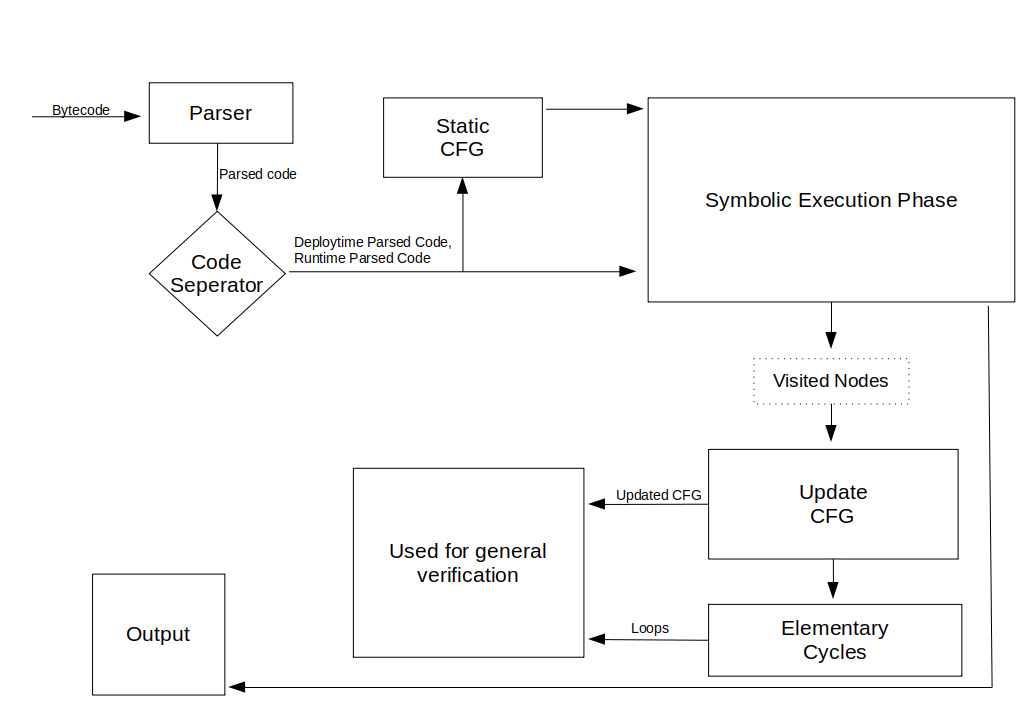
\includegraphics[width = 14cm, height = 12cm]{images/2.png}
\begin{center}
    Figure 2 : Components of DoS Tool
\end{center}

\newpage
\noindent Let's discuss the Components of DoS Tool in detail.\\
\\
\textbf{Parser}\\
Bytecode is hexadecimal representation of the smart contract. EVM(Ethereum Virtual Machine) has predefined opcodes. EVM understand these opcodes. The hexademicals in the bytecode corresponds to these opcodes. For example, \textbf{PUSH1} is an opcode which pushes 1 byte of the data on the stack. The corresponding hexadecimal value is \textbf{'0x60'}. Similarly \textbf{MSTORE} is an opcode which stores data in memory. The corresponding opcode is \textbf{'ox52'} and many more. The size of every opcode is 1 byte. Data in the bytecode can have a maximum of 32 bytes size. PUSH is the only opcode which pushes data into the stack without any computation. Hence such data is given directly in the bytecode in the hexadecimal format right next to the PUSH opcode. For example, the string \textbf{\emph{'6040'}} means \textbf{\emph{60}} corresponds to the PUSH1 opcode where 1 means 1 byte, hence PUSH1 pushes 1 byte of data on the stack. The next one byte, i.e., \textbf{\emph{40}} is the data which PUSH1 will push to the stack. We can find list of EVM opcodes and their corresponding hexadecimal value along with some extra information, such as, gas consumption of the opcode in the Yellow paper of ethereum or on github.\\
\\
The parser takes input the hexadecimal string(bytecode) and returns a list of these opcodes.
The list which parser returns have 4 fields.
\begin{itemize}
    \item \textbf{\emph{step}}: step corresponds to the position in the bytecode string. step is calculated in bytes. for example, let's consider the string '604052'. Here step = 0 means at 0th position in the string. step 1 corresponds to 2nd position in the string and so on. step can be used in the \textbf{JUMP/JUMPI} as an argument of position to jump to.
    \item \textbf{\emph{operand}}: operand is nothing but the hexadecimal value in the bytecode coresponding to the opcode. For example, in the string '604052', 60 is the operand for the opcode PUSH1.
    \item \textbf{\emph{input}}: input is the integer value of the corresponding hexademical data in the bytecode. For example, in the string '604052', the PUSH1(60) needs an input of 1 byte which will be right next to it, i.e., 40 in the string and its integer value is 64.
    \item \textbf{\emph{o}}: o is the opcode corresponding to hexadecimal value of the opcode in the bytecode. For example, in the string '604052', opcode corresponding to '60' is PUSH1 and opcode corresponding to '52' is MSTORE.
    
\end{itemize}
\newpage
\noindent A sample parsed code of an opcode looks like below:\\
\begin{center}
    \textbf{\emph{\{'step' : 2, 'operand' : 60, 'input' : 64, 'o' : PUSH1\}}}
\end{center} 
step equals to 0 means the positions of this opcode is the 2nd byte in the bytecode, operand value at 2nd byte is 60, the input for the operand 60 is 64 and the opcode coresponding to the operand 60 is PUSH1. Hence parser converts bytecode into the custom opcode/assembly code list which we called as parsed code.\\
\\
\textbf{Code Separator}\\
The bytecode is a combination of creation bytecode, we named it as deploytime bytecode and runtime bytecode, we named it as runtime bytecode. The runtime bytecode is the code that is stored on-chain that describes the smart contract. The deploytime bytecode generates the runtime bytecode, it includes contructor logic and constructor parameters. It is equivalent to the input data of the transaction which create smart contract. We have separated deploytime parsed code and runtime parsed code from the parsed code beforehand to feed to the other components of the DoS Tool. A static pattern search is performed to separate these two codes from the bytecode. \textbf{CODECOPY} is an opcode which is used to copy constructor parameters and to copy the runtime bytecode to the memory of the EVM. Also every bytecode, be it deploytime or runtime, starts with fixed instructions. These fixed instruction sets a pointer to the free memory pointer from where the program starts storing data in memory. These instructions are as follows\\
\begin{center}
    PUSH1 mm\\
    PUSH1 dd\\
    MSTORE
\end{center}
Here mm and dd are the hexadecimal 1 byte data for the PUSH1 opcodes. MSTORE needs two inputs the memory location where we want to store, i.e., mm and the data to store at the memory location, i.e., dd. Hence every deploytime bytecode or runtime btecode starts with a string '60mm60dd52'. The algorithm to separate bytcode is as follows\\
\newpage
\begin{Verbatim}[numbers=left,xleftmargin=5mm]
    Search for CODECOPY in the parsed code
    if CODECOPY found
    
        search for RETURN ahead
        if RETURN found
        
            search for the string ahead
            if CODECOPY found
                goto line 2
            if string found
                the parsed code above this position is deploytime bytecode
                the parsed code below from this position is runtime bytecode
                return
            if string NOT found
                return can't separate
                
        if CODECOPY found 
            goto line 2
        if RETURN not found
            return can't separate
            
    if CODECOPY not found
        return can't separate
\end{Verbatim}
\textbf{Static Control Flow Graph}\\
There is an opcode \textbf{JUMPDEST} in the EVM opcode list. The sole purpose of the opcode is to mark the begining of a block. Every block starts with \textbf{JUMPDEST} except the very first block which starts with the magic string '60mm60dd52' as discussed under code separator component. Hence we can obtain list of basic blocks in the parsed code. Now these basic blocks needs to be connected in order to determine the control flow of the program. There are four ways to determine control flow of the program.\\
\begin{itemize}
    \item \textbf{JUMP} opcode: This is an unconditional jump. JUMP only takes one argument which is the destination of the jump. If the destination opcode is JUMPDEST then it is a valid jump else EVM stop traversing this path. When EVM encounters JUMP instruction it takes the current top value of the stack as argument and jumps to this location in the bytecode. This location argument is either directly pushed before JUMP instruction by using PUSH opcode or is a result of some computation, example - add, mul etc. Since we are not executing Custom EVM since, we don't have stack trace and we can only resolve the JUMP location only when its argument is directly pushed by PUSH instruction in the bytecode just before the JUMP instruction.
    \item \textbf{JUMPI} opcode: JUMPI is an conditional jump. JUMPI takes two argument, the top of stack is the jump location and the next value on the stack is a boolean condition value. If condition value is 1 the code jumps to the location provided by jump location argument and if the condition value is 0 the code continue executing without jump. Also if condition value is 1, the jump location in the bytecode is only valid if it is JUMPDEST opcode. JUMPI location can also remain unresolved like the JUMP location.
    \item \textbf{JUMPDEST} opcode: If on execting the current block JUMPDEST instruction is encountered, this is the starting of the next block and control is flowing directly from the current block to the next block. Therefore we simply connects the block with the next adjacent block.
    \item \textbf{INVALID}: If we encounter an INVALID opcode on traversing a block then it is the end of the block and this block is the end block in the path and not connected to any other block  in the control flow of the program.
\end{itemize}
The output of this component is a control flow graph we named as STATIC CFG. The name static is added just to clearify that the control flow of the program is not obtained by executing the program and keeping track of the state trace of the program. There are two shortcomings to the CFG as discussed below.
\begin{itemize}
    \item \textbf{Overestimation of Paths}\\
    To determine static CFG no dynamic or symbolic approach is used. Hence the control flow paths are overestimated because we have considered all paths. There may be possibility that some paths will never be traversed for any inputs during the execution life of the program.
    \item \textbf{Unresolved JUMP/JUMPI}\\
    Even though the Static CFG is overestimated, the CFG may have missed the control flow that is possible to reach during the execution life of the program. This is mainly due to the reason of unresolved JUMP/JUMPI instructions as discussed above.
\end{itemize}
\newpage
\noindent\textbf{Symbolic Execution Phase}\\
The Symbolic Execution Phase will run the bytecode in a Custom EVM symbolically. A diagram of Symbolic Execution Phase is shown in the Figure 3 below.\\
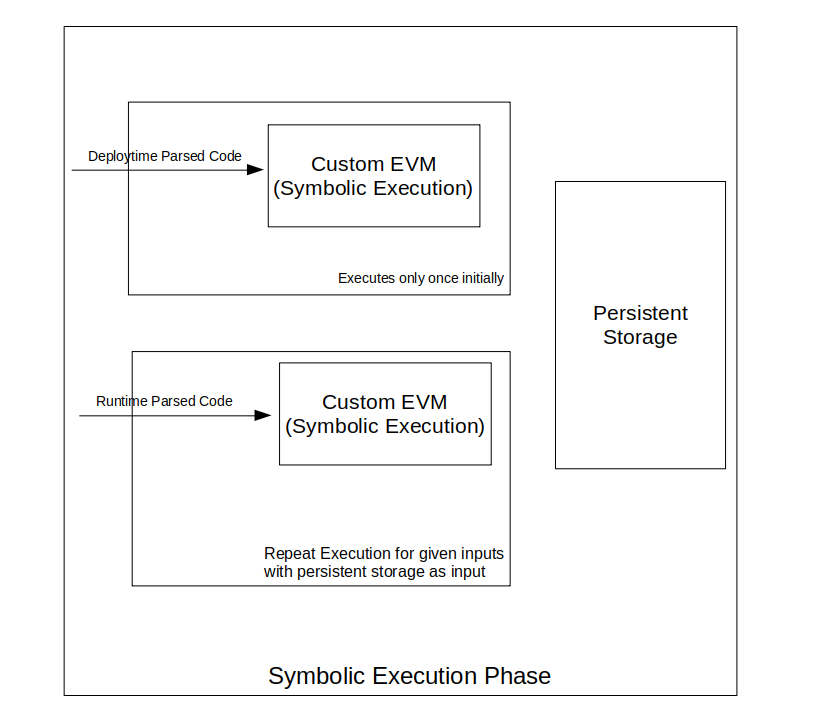
\includegraphics[width = 15cm, height = 14cm]{images/3.png}
\begin{center}
    Figure 3\\
\end{center}
EVM works on the bytecode of the smart contract. EVM is a stack based machine with the maximum limit of the stack is 1024. The EVM generally uses stack for intermediate values in computations. EVM also uses memory and storage other than stack. The memory is the real workhorse and is non-permanent. Storage is used for values which needs to be persists between different executions of the smart contract. Hence storage is permanent. The gas usage of storage is very high as compared to the memory. Hence one should wisely decide between what to store permanently and what should be temporary during smart contract execution. EVM also keeps track of the gas usage in order to terminate program when out of gas. The Custom EVM used in the Symbolic Analysis Phase implements the stack, memory and the storage, basically the state implementation. The Custom EVM don't implement other features of EVM. The idea for the implementation of custom EVM is taken from the tool Maian.\\
The Custom EVM starts executing the parsed code from the start. Any value which can be decided by external user is considered as symbolic. For example, CALLDATA of functions which can be called in order to interact with the smart contracts, the return value from the external smart contracts which were called from the contract, CALLVALUE - the value of ether send to a payable function by the external user. Upon traversing the exectuion path, these symbolic variables build symbolic expressiions. When the control flow branches we use SMT solver to decide whether the further path is feasible of not. If the SMT solver returns not satisfiable for the certain path condition then it will not be traversed. We have taken few design choices in order to migigate some of the problems as discussed below. 
\begin{itemize}
    \item \textbf{Infinite Loops}: Infinite loop detection is undecidable. Therefore during the execution of the Custom EVM, there may be possibility that the execution never stops. Hence we introduced maximum path length from the start of the execution. When the execution arrives at the new block the path length increases by one and if a certain path length reaches maximum path length limit the Custom EVM reverts and stops traversing the path. There is no way to decide what should be the appropriate value of maximum path length. Hence we tested the tool on three maximum path length, i.e, 10, 20 and 40. The maximum path length is given as input to the tool by the user.
    \item \textbf{Multiple Invocation of smart contracts}: Let's understand this with an example.
    \begin{Verbatim}[numbers=left,xleftmargin=5mm]
    pragma solidity ^0.4.24;
    contract BasicToken {
        uint256[] balances;
        function balanceOf() public  view returns (uint256) {
            uint c = 1;
            balances.push(a);
            return c;
        }
        function print() public view returns (uint256){
            uint256 temp = 0;
            for(uint256 i = 0; i < balances.length; i++){
                temp += balances[i];
            }
        return temp;
        }
    }
    \end{Verbatim}
    It is necessary to know how bytecode calls external function. The first 4 bytes of the keccak of the external function known as function signature are the identifier of functions in the bytecode.
    for example the function signature of \emph{print()} function in the above code will be '13bdfacd' and function signature of \emph{balanceOf()} function in the the code will be '722713f7'. The assembly view of external functions in the smart contract above is
    \begin{Verbatim}[numbers=left,xleftmargin=5mm]
        PUSH4 0x13BDFACD 
	EQ 
	PUSH2 0x51 
	JUMPI 
	DUP1 
	PUSH4 0x722713F7 
	EQ 
	PUSH2 0x7C 
	JUMPI
    \end{Verbatim}
    Hence the first for byte of the CALLDATA will be compared with the function signature and jump to the corresponding function block. Since our Custom EVM starts executing bytecode from the start, first the \emph{print()} function will be executed and then the \emph{balanceOf()} function. The loop condition in the \emph{print()} function is symbolic because of the \emph{balanceOf()} function. Hence balances.length will be set to symbolic when the Custom EVM executes \emph{balanceOf()} function. Therefore in the first invocation of the smart contract the vulnerability will not be captured. But since the balances.length is stored in the storage and we know storage is persistent, in the second invocation of the smart contract, even on executing the \emph{print()} function first again, the vulnerability will be captured because the balances.length was set to symbolic in the previous invocation of the CUstom EVM. Hence the tool should test on multiple invocations of the smart contract in order to capture such vulnerabilites. We have test on invocations 1 and 2 but this is also given as argument to the Custom EVM.
    \item \textbf{Constant Loops with iterations more than MAXIMUM PATH LENGTH}\\
    In constant loop the loop condition is constant and hence SMT solver can do nothing much but will traverse the loop iteration until loop completes. Only after completion of loop the path after the loop in the program will be traversed. Hence he branch of execution after a constant loop is only accessible after the completion of loop. Hence if a constant loop is terminated in between the path after the loop will never be traversed. Although we have made this design choice by keeping in mind that all paths will not be traversed for the cost of not trapping into the infinite loop. But we can break this constant loop early and since we know that loop condition is constant we can traverse the path after the loop instead of looping the maximum path length into the constant loop.
    This should also be noticed that these constant loops can also exceeds the block gas limit. So only constant loops for 10000 iterations are considered for our Custom EVM. EVM block gas limit in practice exceeds for loops around 2-4 lakhs of iterations. Again this can be set and not fixed in the Custom EVM.
\end{itemize}
Th Static CFG is also an input to the Symbolic Execution Phase to resolve the unresolved control flow paths as discussed in the Static CFG. We have also maintained a list of visited nodes. Whenever a new block is reached at any point in the exectution, on any invocation we add it to the visited list. Hence visited node is a list of blocks ever visited during the Symbolic Execution phase of the DoS Tool.\\
\\
\textbf{OUTPUT}\\
The symbolic Execution Phase outputs the vulnerability of the smart contract from the four vulnerabilities as discussed above and as safe if no vulnerability is found.\\
\\
\textbf{Update CFG and Elementary Loops}\\
The updated CFG will used the visited nodes list updated by Symbolic Execution Phase as input. Update CFG will remove nodes and their paths from the Static CFG. Hence the number of paths in updated CFG are suby cuvion/-
s-+
ets of the path in the Static CFG. The number of paths corresponding to the Static CFG and Updated CFG are showwn in the output of the DoS Tool.\\
The elementary loops will find all the elementary loops in the updated CFG. It is to be noted that the loops found during the symbolic analysis phase are different from the loops obtained from the Updated CFG. After careful observation we noticed that the loops obtained during Symbolic Execution should be subset of the loops obtained from the Static CFG. There may be many reasons for this and we will see on reason with the help of Graph 1. Let the contract execution starts from node A and we will consider only 1 invocation of the smart contract. Suppose the control flow AC is not symbolically feasible during the execution of the smart contract. The execution can traverses path AB or ABC or ABCD or ABCDA. If we the execution goes all the way back to the A by traversing path ABCDA, then all the nodes will be in the visited nodes list. Hence the Static CFG and the Updated CFG will be same because we considered all visited nodes without considering whether the path from one node to another is actually feasible or not.\\
\begin{center}
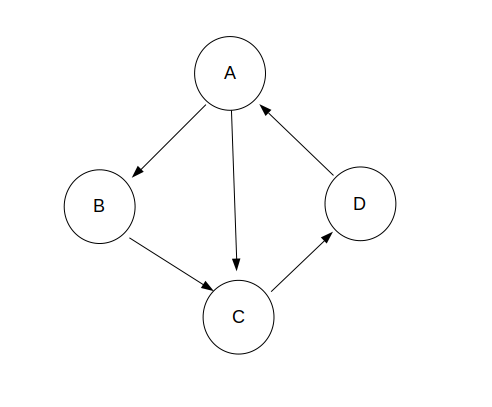
\includegraphics[width=10cm, height=7cm]{images/4.png}.

    Graph 1
\end{center}
Hence when we find loops using graph algorithm on the Updated CFG, we will get two loops ABCDA and ACDA, while the Symbolic Analysis Phase returns only 1 loop, i.e., ABCDA. These features are not necessary for the tools but we build these components in order to do some reasoning about the DoS Tool.

\newpage
\section*{Chapter 5}
\section*{Results}
The tool is setup on a 64-bit Ubuntu 20.04 LTS, 7.7 GB of RAM and 8 Core Intel(R) Core(TM) i5-8250U CPU @ 1.60GHZ. A Total of 35 smart contracts are tested with 6 different sets of \{Invocations, Path length\}. We have tested the tool on 1 and 2 invocations with path length 10, 20 and 40 respectively for each of the mentioned invocations.
The result of the tool for 1 invocation and sets of path length is shown in the Chart 1.\\
\\
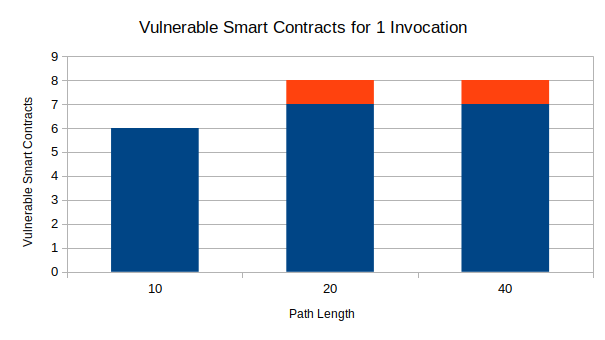
\includegraphics[width= 15cm]{images/51.png}
\begin{center}
    Chart 1
\end{center}
A total of 6 smart contracts are flagged as vulnerable in the setup with 1 invocation and path length equals to 10. A total of 7 smart contracts are flagged as vulnerable in the setup with 1 invocation and path length equals to 20. Out of those 7 smart contracts. 1 smart contract is false positive. The result with 1 invocation and path length 40 path length is same as the 1 invocation and 20 path length.\\
\\
The result of the tool for 2 invocations i s shown in the Chart 2. A total of 9 smart contracts are flagged as vulnerable in the setup with 2 invocation and path length equals to 10. A total of 11 smart contracts are flagged as vulnerable in the setup with 2 invocation and path length equals to 20. Out of those 11 smart contracts, 1 smart contract is false positive. The result with 2 invocation and path length 40 path length is also the same as the 2 invocation and 20 path length. 
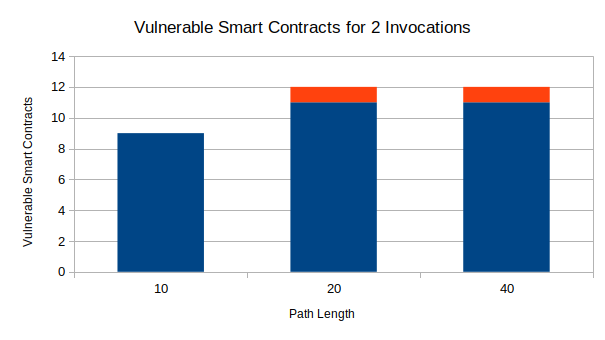
\includegraphics[width = 15cm]{images/52.png}
\begin{center}
    Chart 2
\end{center}
The 2 invocation setup was able to find more vulnerable contract which otherwise was left by the 1 invocation setup. This was expected as we have explained in Symbolic Execution Phase of the Dos Tool. Also with the increase in number of path length the tool was able to traverse path more deeply and explore more vulnerabilities if present. A comparison chart with different invocation setup and path length is shown in Chart 3.\\
\\
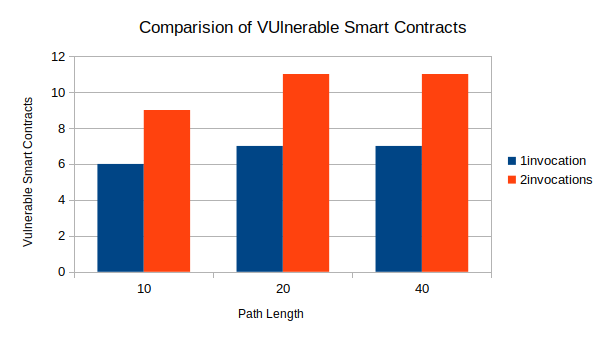
\includegraphics[width= 16cm]{images/53.png}
\begin{center}
    Chart 3
\end{center}
\subsection*{About the False Positive Case}
The false positive case is for the vulnerability of unbounded loop condition. We have assumed that the symbolic value can take any value. For the example consider this value as the integer value. Now the integer type variable have different ranges based on the type of integer in solidity. For example solidity have signed and unsigned integer of different sizes. The range varies from 8 bit number to 256 bit number with keywords : unint8 to unint256 and int8 to int256. An unsigned integer uint32 has a range from 0 to 2**32 - 1. \\
But SMT solver on symbolic expressions yield same result of all different ranges of integer value in the loop condition and we have given the range limit of 256 bit number for the SMT Solver. We need to know different range of integers which with the current tool is not possible to determine and the SMT will overestimate paths based on our current setup. The smart contract which gives false positive looks like below:
\begin{Verbatim}[numbers=left,xleftmargin=5mm]
    function nameFilter(string _input)
        returns(bytes32)
    {
        uint256 _length = _temp.length;
        require (_length <= 32 && _length > 0);
        for (uint256 i = 0; i < _length; i++)
        {
            //some code
        }
    }
\end{Verbatim}
Although the \emph{\_input} length is symbolic since the string is symbolic. Its length is limited by the line number 5 of the code. But the SMT will return satisfiable for the Symbolic expression in the loop condition at line 6. These limitations based on integer size or checks as performed in the above code are falsely interpreted as vulnerable contracts by the tool.

\newpage
\section*{Chapter 6}
\section*{Summary and Future Work}
\subsection*{Summary}
In this thesis we develop a symbolic analysis tool for checking whether a smart contract is vulnerable for denial of service vulnerabilities or not. We start by looking at denial of service vulnerabilities in smart contract discovered already in the past. We deduced some patterns because of which those vulnerabilities were possible. We then go on to explain the tool and various components in the tool. We explained some designed choices in order for the successful execution of the tool. We then discuss the results and some details about the shortcoming of the tool, where the tool will fail. \\
\subsection*{Future Work}
\begin{itemize}
    \item We can build a type checking module that works alongside of the code in order to help SMT solver to decide what range to check instead of checking fixed range values.
    \item One can think of extending the tool for more patterns of Dos attacks which can be found in future.
    \item The tool is detecting whether smart contract is vulnerable and that vulnerability arises from which external function using the function signature. But we have only used function signature which are keccak256 of the functions in solidity. We can also join bytecode to source code converter module to exactly determine the functionality of the function that is causing the vulnerability.
    \item This tool is specifically made for checking vulnerabilities in ethereum smart contracts. Similar approach can be followed for other smart contracts available. 
\end{itemize}
\newpage
\section{Bib}
\end{document}
